% CVPR 2026 Paper Template; see https://github.com/cvpr-org/author-kit

%%% Outline %%%%
%%% Abstract: What is the scientific question we are answering

%%% Intro: 

%%%% Related Work: ASD vallence arousal detection from stimming behavior.

%%%% Methodology: 
% 1. Dataset + Annotation: SSDB +ASBD
% 2. Briefly Benchmark description: Emotic? (limitation: no ASD specific dataset to pre-train or benchmark)
% 3. Architecture

%%% Evaluation: Model comparision, Bechmark comparision, Ablation
%%% Results & Discussion: 
%%% Conclusion


% Nov 10 Result Discusssion
% Conclusion: Pose has to be argued about

% 1 straem
% Pose is not improving arousal (less than random)
% Face is giving decent valence
% VLM description is giving best Arousal (valence same)
% Event annotation impproves both

% 2 streams
% Pose detoriate event annotation result.
% Pose + face further low ressult
% Annotation + face bolster the result - best
% VLM + facce - increases accuracy

% 3 stream
% PPose reduces performance
% best model is VLM + face + annotation
% 

\documentclass[10pt,twocolumn,letterpaper]{article}



%%%%%%%%% PAPER TYPE  - PLEASE UPDATE FOR FINAL VERSION
% \usepackage{cvpr}              % To produce the CAMERA-READY version
\usepackage[review]{cvpr}      % To produce the REVIEW version
% \usepackage[pagenumbers]{cvpr} % To force page numbers, e.g. for an arXiv version

% Import additional packages in the preamble file, before hyperref
%% This file contains a number of tweaks that are typically applied to the main document.
%% They are not enabled by default, but can be enabled by uncommenting the relevant lines.

%%
%% Inline annotations; for predefined colors, refer to "dvipsnames" in the xcolor package:
%% https://tinyurl.com/overleaf-colors
%%
\newcommand{\red}[1]{{\color{red}#1}}
\newcommand{\todo}[1]{{\color{red}#1}}
\newcommand{\TODO}[1]{\textbf{\color{red}[TODO: #1]}}


%%
%% disable for camera ready / submission by uncommenting these lines  
%%
% \renewcommand{\TODO}[1]{}
% \renewcommand{\todo}[1]{#1}

%%
%% work harder in optimizing text layout. Typically shrinks text by 1/6 of page, enable
%% it at the very end of the writing process, when you are just above the page limit
%%
% \usepackage{microtype}

%%
%% fine-tune paragraph spacing
%%
% \renewcommand{\paragraph}[1]{\vspace{.5em}\noindent\textbf{#1.}}

%%
%% globally adjusts space between figure and caption
%%
% \setlength{\abovecaptionskip}{.5em}


%%
%% Allows "the use of \paper to refer to the project name"
%% with automatic management of space at the end of the word
%%
% \usepackage{xspace}
% \newcommand{\paper}{ProjectName\xspace}

%%
%% Commonly used math definitions
%%
% \DeclareMathOperator*{\argmin}{arg\,min}
% \DeclareMathOperator*{\argmax}{arg\,max}

%%
%% Tigthen underline
%%
% \usepackage{soul}
% \setuldepth{foobar}

%%
%% ContextPose figure and notation (methodology_h.tex)
%%
\usepackage{bm}
\usepackage{tabularx}
\usepackage{tikz}
\usetikzlibrary{positioning,arrows.meta,calc,fit,backgrounds}

\tikzset{
  box/.style={draw,rounded corners=2pt,align=center,font=\footnotesize,minimum height=7mm,inner sep=3pt,fill=white},
  inp/.style={box,fill=blue!6},
  op/.style={box,fill=gray!8},
  outputnode/.style={box,fill=green!8},
  arr/.style={-{Stealth[length=2mm]},thick},
  winframe/.style={draw=gray!65,dashed,rounded corners=3pt,inner sep=5pt},
  faceframe/.style={draw=orange!70!black,dashed,rounded corners=3pt,inner sep=5pt},
  framelabel/.style={font=\scriptsize,align=center,fill=white,inner sep=1pt},
}

\newcommand{\R}{\mathbb{R}}
\newcommand{\regions}{\mathcal{R}}
\newcommand{\vc}{\mathbf{c}}
\newcommand{\vchat}{\hat{\mathbf{c}}}
\newcommand{\ve}{\mathbf{e}}
\newcommand{\vq}{\mathbf{q}}
\newcommand{\vsum}{\mathbf{s}} % \vs is taken by cvpr.sty ("vs.")
\newcommand{\vh}{\mathbf{h}}
\newcommand{\vy}{\hat{\mathbf{y}}}
\newcommand{\vb}{\mathbf{b}}
\newcommand{\vu}{\mathbf{u}}
\newcommand{\mZ}{\mathbf{Z}}
\newcommand{\mX}{\mathbf{X}}
\newcommand{\mS}{\mathbf{S}}
\newcommand{\mW}{\mathbf{W}}
\newcommand{\GELU}{\operatorname{GELU}}
\newcommand{\ReLU}{\operatorname{ReLU}}
\newcommand{\LN}{\operatorname{LN}}
\newcommand{\Drop}{\operatorname{Drop}}
\newcommand{\softmax}{\operatorname{softmax}}


% It is strongly recommended to use hyperref, especially for the review version.
% hyperref with option pagebackref eases the reviewers' job.
% Please disable hyperref *only* if you encounter grave issues, 
% e.g. with the file validation for the camera-ready version.
%
% If you comment hyperref and then uncomment it, you should delete *.aux before re-running LaTeX.
% (Or just hit 'q' on the first LaTeX run, let it finish, and you should be clear).
\definecolor{cvprblue}{rgb}{0.21,0.49,0.74}
\usepackage[pagebackref,breaklinks,colorlinks,allcolors=cvprblue]{hyperref}

%%%%%%%%% PAPER ID  - PLEASE UPDATE
\def\paperID{*****} % *** Enter the Paper ID here
\def\confName{CVPR}
\def\confYear{2026}

%%%%%%%%% TITLE - PLEASE UPDATE
\title{Event-Centric Multimodal Affective Repressentation Learning from Self-Stimulatory Behaviors in Autism.}

%%%%%%%%% AUTHORS - PLEASE UPDATE
\author{First Author\\
Institution1\\
Institution1 address\\
{\tt\small firstauthor@i1.org}
% For a paper whose authors are all at the same institution,
% omit the following lines up until the closing ``}''.
% Additional authors and addresses can be added with ``\and'',
% just like the second author.
% To save space, use either the email address or home page, not both
\and
Second Author\\
Institution2\\
First line of institution2 address\\
{\tt\small secondauthor@i2.org}
}

\begin{document}
\maketitle
\input{0_abstract}  

\input{sec/1_intro}
\section{Introduction [0.8 page approx]}
\label{sec:intro}

[0.8 page approx]
%Added Text by: Olivia
Affect identification in mental disorders has been a topic recently being studied in the machine learning realm [2]. Stimming behaviors (or motor stereotypies), that are commonly seen in ASD youth, can be considered hard to categorize, and a complex feature of their affective behavior. Machine learning has been helpful in assisting with diagnosis and other related application needs. The purpose of machine learning in this manner is to assist clinicians in evaluating and diagnosing certain affects that may be present. There exists a gap in the data readily available to use for stimming, due to confidentiality and privacy matters, as the manner of conducting information would have to be through children. The problem also lies in social behaviors and language abilities are mostly seen interpersonally through observation[1]. Because of these gaps, using images to aid machine learning training has proven to be helpful, as there are a multitude of factors that can be accounted for in analysis, such as behavior and facial recognition. However, videos to evaluate ASD behaviors due to children having free range of motion and being able to act naturally in the environment can be the closest to real-life observation. Previous literature has been more focused on the evaluation and diagnostic criteria for ASD individuals, and not the treatment or observation of behaviors after the fact. Studying affect in ASD children can help researchers and clinicians further understand how the child may be feeling or thinking, in order to have a greater grasp on the disorder [2].

\subsection{Motivation and Research Context}
ASD is a mental disability that can be characterized by deficits in several cognitive facets, such as speech, comprehension and motor abilities. The diagnostic rate has risen over time, most likely due to the fact that critical attributes are more well known in the greater population. There is no reliable way to test before birth if a child has predisposition to ASD; however, early diagnosis is key to getting meaningful intervention that will help the child. Conducting observations specifically looking at social behaviors and expressive language can further delay a diagnosis, which people can spend months on a waiting list for. “Self-stimulatory behaviors" or stimming is characterized by repetitive behavior that is observed to be used for many different feelings in children with ASD: negative, positive or simply for sensation purposes. “Human recognition models” that have been created in recent years have shown great promise in being able to detect what it is programmed to look for, such as certain periodic or sustained stimming behaviors such as “gaze aversion, hand flapping, or headbanging”. Training models to be able to identify these behaviors can be advantageous in seeing patterns that the human brain cannot comprehend. Being able to identify “symptomatic events” before stimming behaviors happen can be helpful for therapeutic remedies for the child [1].
%End Text: Olivia

\subsection{Research Gap}

Stereotypical movements associated with autism spectrum disorder (ASD), such as arm flapping, head banging, and spinning, are often assessed manually, making measurement time-consuming and difficult to scale. Although automated recognition systems exist, potential data leakage from splitting clips from the same video across training and test sets may inflate performance. Evaluation on unseen videos remains limited, and few studies fairly compare privacy-preserving pose-based models with RGB-based models and handcrafted motion features.

Existing research also provides limited insight into movement changes before behavior onset and their associations with observable contextual events, such as social interactions, auditory events, and activity changes. Additionally, it remains unclear whether ASD-relevant upper-body movement patterns are associated with observer-rated valence and arousal or can partially predict these ratings. These ratings reflect perceived affect rather than a child's internal emotional state.

This work addresses these gaps through leakage-free behavior recognition benchmarking, comparisons of pose-based, handcrafted, and RGB-based approaches, analysis of pre-onset movement and contextual associations, and an exploratory investigation of observer-rated affect without implying causation.

\subsection{Research Hypotheses}

\begin{itemize}
    \item \textbf{H1: Behavior Recognition.} Temporal pose-based models can distinguish among the four stereotypical behavior categories more effectively than simple handcrafted motion statistics that summarize movement intensity.

    \item \textbf{H2: Precursor Movement Changes.} Measurable changes in movement occur before stereotypical behavior onset, relative to ordinary, non-event periods from the same video footage.

    \item \textbf{H3: Context Association.} Pre-onset movement changes are associated with observable contextual events, including social interactions, auditory events, activity or object changes, and visual or screen-based events.

    \item \textbf{H4: Observer-Rated Affect (Exploratory).} Episode-level observer-rated affect, expressed in terms of valence (the apparent positivity or negativity of the child's affect) and arousal (the apparent level of activation or calmness), is associated with pre-onset movement changes, and aspects of these ratings can be partially recovered from upper-body movement alone.
\end{itemize}

H1 evaluates behavioral classification, while H2 and H3 examine pre-onset movement changes and their associations with observable context, without implying causation. H4 is exploratory because valence and arousal ratings were added after the original study design. Three observers, blinded to the study results, rated each clip as a whole. Therefore, these ratings characterize episode-level perceived affect rather than the child's internal emotional state or affect specifically before behavior onset. H4 examines associations between these episode-level ratings and pre-onset movement changes.

\noindent\textbf{Contributions.}
\begin{enumerate}
    \item A pose-based pipeline for four stereotypy categories, evaluated using video-grouped cross-validation against a handcrafted-feature baseline.
    \item An analysis of movement dynamics around behavior onset across pre-event, event, and post-event windows.
    \item A context annotation scheme and an analysis of how contextual events relate to subsequent movement.
\end{enumerate}

% Spans both columns (best for this wide 4x3 diagram)
\begin{figure*}[t]
  \centering
  \includegraphics[width=\textwidth]{fig/end_to_end_pipeline.png}
  \caption{End-to-end pipeline. Annotated ASD videos are segmented into behavior episodes, split by video, and converted to cleaned 2D pose sequences (YOLO11 + ByteTrack, ViTPose++). These are classified with handcrafted-feature or deep temporal models, and a Pre/Event/Post window analysis on context clips examines movement changes around behavior onset.}
  \label{fig:pipeline}
\end{figure*}

\input{sec/2_relatedwork}
\input{sec/3_material_methods}
\section{Dataset and Annotation}
\label{sec:data}

Data curation, event timestamps, subject-level splits, context annotation, and research tasks.\\
Describe the sources, inclusion criteria, available videos, unusable records, behavior labels, and event timestamps. Report the actual final counts after curation rather than using preliminary counts as final results.

\subsection{Dataset Sources and Curation}
\label{subsec:dataset_curation}
% TODO: sources, inclusion criteria, final counts after curation (videos, clips, subjects),
% unusable records, behavior labels (arm flapping, hand flapping, head banging, spinning), timestamps.

\begin{figure}[t]
  \centering
  \includegraphics[width=\columnwidth]{fig/video_split_and_context_clip.png}
  \caption{(a) Video-level split: all segments of a source video stay together (blue/orange blocks), in the same split and stratified by behavior class. (b) Construction of an event-centred context clip (\texttt{--window 5}) and the subsets A and B. Here $\mathrm{pre}_s = \mathrm{start}_1$ (first segment) or $\mathrm{start}_i - \mathrm{end}_{i-1}$ (later segments), and $\mathrm{post}_s = \mathrm{duration} - \mathrm{end}$. Subset~A contains all usable segments; Subset~B requires $\mathrm{pre}_s \ge 5$\,s ($B_{\mathrm{pre}}$) and $\mathrm{post}_s \ge 5$\,s ($B_{\mathrm{pre\_post}}$).}
  \label{fig:split_context}
\end{figure}

\subsection{Event Definition and Temporal Windows}
\label{subsec:event_temporal_windows}
For each annotated behavior we define three windows: \emph{pre-event} (the 10\,s before the behavior begins), \emph{event} (the annotated behavior interval), and \emph{post-event} (the period after the behavior ends, limited by video availability). A 5\,s pre-event window serves as a sensitivity analysis. 
% TODO: overlapping events, timestamp uncertainty, short clips.

\subsection{Context Annotation}
\label{subsec:context_annotation}
Three annotators independently and blindly labeled each of 192 context clips (92 videos) for four binary contextual events: social interaction, auditory event, activity/object change, and visual/media event. A fifth field, \emph{No Event}, is $1$ only when all four indicators are $0$. Each judgment carries a confidence score from 1 to 5. Annotators also rated the emotional effect on a valence scale (positive, neutral, negative, unknown) and an arousal scale (high, low, unknown) (Fig.~\ref{fig:context-annotation}).

Binary fields are resolved by majority vote. Valence and arousal are mapped to $[-1,1]$ (valence: positive $+1$, neutral $0$, negative $-1$; arousal: high $+1$, low $-1$; unknown $0$) and combined by a confidence-weighted mean
\begin{equation}
\hat{y}_d=\frac{\sum_{i\in S_d} w_{i,d}\,y_{i,d}}{\sum_{i\in S_d} w_{i,d}},\qquad w_{i,d}=c_{i,d}/5,
\end{equation}
where $S_d$ is the set of annotators with a rating for dimension $d$ and $c_{i,d}$ is the confidence score.

\begin{figure}[t]
    \centering
    \includegraphics[width=1.0\linewidth]{fig/clip_to_annotation.png}
    \caption{Context annotation. Each clip is split into pre- and post-event windows, and annotators label four contextual events and the emotional effect (valence, arousal), each with a confidence score.}
    \label{fig:context-annotation}
\end{figure}

\paragraph{Annotator agreement.}

\input{table/annotator_agreement2}
Table~\ref{tab:agreement} reports agreement among the three annotators. Agreement is highest for visual/media events and weakest for activity/object change and arousal. For fields where one label dominates (auditory event, no event), Fleiss' $\kappa$ is low despite high raw agreement, so we also report Gwet's AC1.
% [paste your agreement table here]



\section{Context Pose}
\label{sec:method}

ContextPose estimates the valence and arousal reflected in human annotations of short video clips depicting a child before, during, and after an environmental event. The proposed architecture is motivated by the hypothesis that contextual information can help identify the behavioural moments most relevant to an affective response. Rather than merely concatenating context with an aggregated behaviour feature, we use the context representation as an attention query over the temporal behaviour features. In this formulation, context determines how the behaviour sequence is summarised, while the attended values themselves are derived from the child's observed behaviour.

The framework is illustrated in Figure~\ref{fig:arch}. The child's behaviour is described by one of two interchangeable inputs: body-pose features computed from tracked joints, or subject-aware frame embeddings computed directly from the video by EmotionCLIP. Whichever input is used, the sequences from the pre-event, event, and post-event intervals are first encoded independently using a shared temporal convolutional network. Event context, represented either through annotations or a language-based description, is mapped into the same latent space. For each interval, the context embedding is combined with a learned region embedding to query the corresponding temporal behaviour tokens using multi-head cross-attention. The resulting three summaries are integrated by a single-layer Transformer and passed to a prediction head for valence and arousal. When reliable facial observations are available, an auxiliary face branch provides an additive correction.

\begin{figure*}[t]
\centering
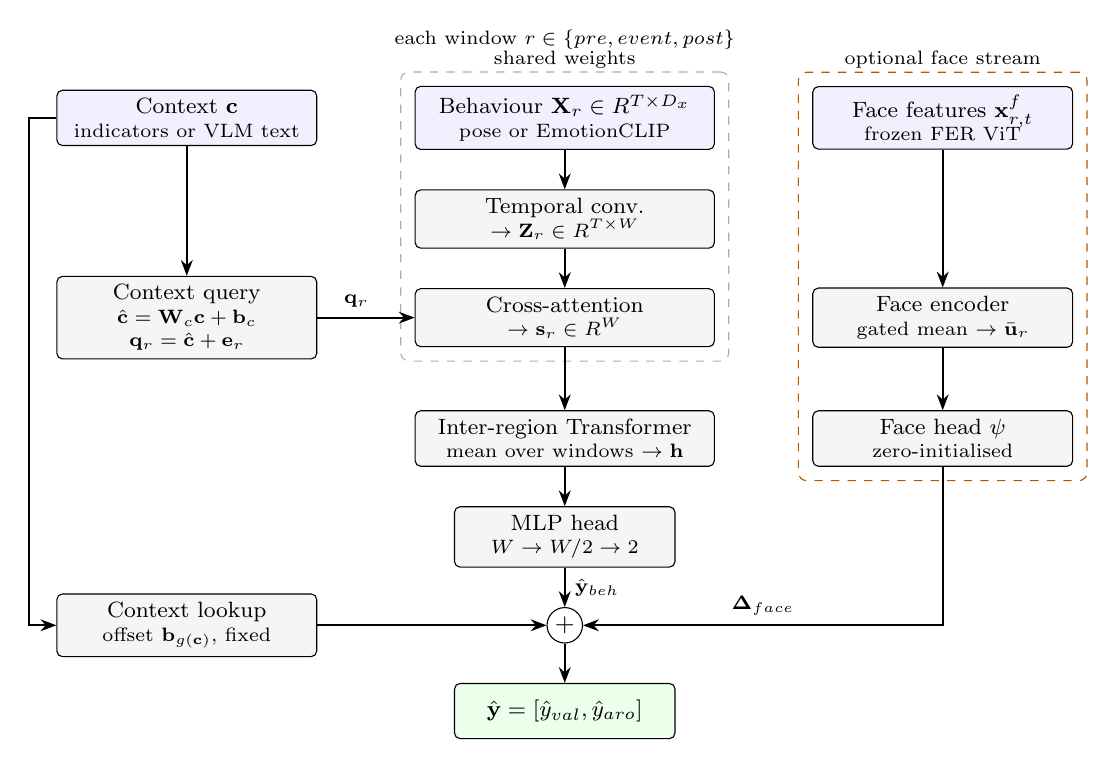
\begin{tikzpicture}[node distance=5mm]
  % Behaviour stream for one window r; the frame marks modules shared by the three windows
  \node[inp,minimum width=3.8cm] (X) {Behaviour $\mX_r\in\R^{T\times D_x}$\\[-1pt]{\scriptsize pose or EmotionCLIP}};
  \node[op,minimum width=3.8cm,below=of X] (T) {Temporal conv.\\[-1pt]{\scriptsize $\to\mZ_r\in\R^{T\times W}$}};
  \node[op,minimum width=3.8cm,below=of T] (A) {Cross-attention\\[-1pt]{\scriptsize $\to\vsum_r\in\R^{W}$}};
  \begin{scope}[on background layer]
    \node[winframe,fit=(X)(T)(A)] (win) {};
  \end{scope}
  \node[framelabel,anchor=south] at (win.north) {each window $r\in\{\text{pre},\text{event},\text{post}\}$\\[-1pt]shared weights};
  \draw[arr] (X) -- (T);
  \draw[arr] (T) -- (A);

  % Fusion and output
  \node[op,minimum width=3.8cm,below=8mm of A] (RT) {Inter-region Transformer\\[-1pt]{\scriptsize mean over windows $\to\vh$}};
  \node[op,minimum width=2.8cm,below=of RT] (H) {MLP head\\[-1pt]{\scriptsize $W\to W/2\to 2$}};
  \node[draw,circle,inner sep=0pt,minimum size=4.5mm,font=\small,below=of H] (plus) {$+$};
  \node[outputnode,minimum width=2.8cm,below=of plus] (Y) {$\vy=[\hat y_{\text{val}},\hat y_{\text{aro}}]$};
  \draw[arr] (A) -- (RT);
  \draw[arr] (RT) -- (H);
  \draw[arr] (H) -- node[right,font=\scriptsize]{$\vy_{\text{beh}}$} (plus);
  \draw[arr] (plus) -- (Y);

  % Context: query for the cross-attention, and key for the fixed lookup offset
  \node[inp,minimum width=3.3cm] (C) at ($(X)+(-4.8,0)$) {Context $\vc$\\[-1pt]{\scriptsize indicators or VLM text}};
  \node[op,minimum width=3.3cm] (Q) at (C |- A) {Context query\\[-1pt]{\scriptsize $\vchat=\mW_c\vc+\vb_c$}\\[-1pt]{\scriptsize $\vq_r=\vchat+\ve_r$}};
  \node[op,minimum width=3.3cm] (Lk) at (C |- plus) {Context lookup\\[-1pt]{\scriptsize offset $\vb_{g(\vc)}$, fixed}};
  \draw[arr] (C) -- (Q);
  \draw[arr] (Q.east) -- node[pos=0.4,above,font=\scriptsize]{$\vq_r$} (Q.east -| A.west);
  \draw[arr] (C.west) -- ++(-3.5mm,0) |- (Lk.west);
  \draw[arr] (Lk.east) -- (plus.west);

  % Optional face stream
  \node[inp,minimum width=3.3cm] (F) at ($(X)+(4.8,0)$) {Face features $\mathbf{x}^{f}_{r,t}$\\[-1pt]{\scriptsize frozen FER ViT}};
  \node[op,minimum width=3.3cm] (FE) at (F |- A) {Face encoder\\[-1pt]{\scriptsize gated mean $\to\bar{\vu}_r$}};
  \node[op,minimum width=3.3cm] (FH) at (F |- RT) {Face head $\psi$\\[-1pt]{\scriptsize zero-initialised}};
  \begin{scope}[on background layer]
    \node[faceframe,fit=(F)(FE)(FH)] (face) {};
  \end{scope}
  \node[framelabel,anchor=south] at (face.north) {optional face stream};
  \draw[arr] (F) -- (FE);
  \draw[arr] (FE) -- (FH);
  \draw[arr] (FH.south) |- node[pos=0.75,above,font=\scriptsize]{$\bm{\Delta}_{\text{face}}$} (plus.east);
\end{tikzpicture}
\caption{ContextPose. Each window's behaviour sequence (pose features or subject-aware EmotionCLIP embeddings) is encoded by a temporal convolution and summarised by cross-attention, with a query formed from the projected context and a learned region embedding. The framed modules share their weights across the three windows. A Transformer layer relates the three window summaries, which are averaged and decoded to valence and arousal. The output is a residual on a fixed context-lookup offset, and the optional face stream (dashed) adds a zero-initialised correction.}
\label{fig:arch}
\end{figure*}

\subsection{Problem formulation and inputs}
\label{sec:inputs}

We organise each clip into three event-centred intervals, indexed by $r\in\regions=\{\text{pre},\text{event},\text{post}\}$: a 5\,s pre-event interval, the event interval itself, and a 5\,s post-event interval. Clips lasting 10\,s or less are omitted because they contain no event frames under this partition. Each interval is resampled to $T=32$ temporal steps, and its behaviour input is a sequence of step vectors $\mX_r\in\R^{T\times D_x}$, built either from pose or from EmotionCLIP as described below. The overall clip is associated with an event-context vector $\vc\in\R^{d_c}$. If the facial branch is active, each interval additionally provides face embeddings $\mathbf{X}^f_r\in\R^{T\times D}$ and a binary validity mask $\mathbf{m}_r\in\{0,1\}^{T}$. The network outputs two unconstrained values $\vy\in\R^2$, corresponding to valence and arousal, whose interpretation is specified by the selected learning objective.

\paragraph{Pose input.}
We retain $J=11$ upper-body COCO landmarks (nose, eyes, ears, shoulders, elbows, and wrists), tracked at $f_s=25$\,fps. Let $\mathbf{p}_{n,j}\in\R^2$ denote joint $j$'s image coordinates in frame $n$. To reduce sensitivity to camera position and apparent subject scale, coordinates are centred at the shoulder midpoint $\mathbf{o}_n$ and normalised by the clip-level median shoulder width $w$:
\begin{equation}
  \tilde{\mathbf{p}}_{n,j} = \frac{\mathbf{p}_{n,j}-\mathbf{o}_n}{w}.
\end{equation}
Each joint contributes four features: two normalised coordinates, detector confidence clipped to $[0,1]$, and movement speed in shoulder widths per second. Missing detections receive zero coordinates and confidence. For each of the $T=32$ resampled steps, interpolation uses both surrounding observations when available, the single available observation otherwise, and zero when neither is available. This avoids inventing trajectories across gaps while retaining confidence as an indication of detection quality.

We compute speed from the original frames before resampling, since resampling intervals of different durations to the same number of steps would otherwise discard real-time movement rate:
\begin{equation}
  v_{n,j} = \min\!\left(f_s\,\lVert\tilde{\mathbf{p}}_{n,j}-\tilde{\mathbf{p}}_{n-1,j}\rVert_2,\; v_{\max}\right), \qquad v_{\max}=20.
\end{equation}
When the preceding observation is unavailable, the next valid observation is used; if neither is available, speed is zero. The cap reduces sensitivity to tracking errors. At each resampled step, speed is averaged over observed frames in a centred span of approximately $N_r/T$ original frames, where $N_r$ is the interval length, preserving a consistent real-time interpretation across intervals.

\paragraph{Subject-aware video input.} Alternatively, each step is described directly from the video by EmotionCLIP (Zhang et al., 2023), a CLIP ViT-B/32 image encoder trained on vlog videos and their transcripts to represent the emotional state of a designated person. EmotionCLIP is subject-aware: alongside the RGB frame, it receives a binary mask marking the person to be read, which is average-pooled over each $32\times32$ patch and added to that patch's positional embedding. The encoder therefore attends to the subject's body and face while still seeing the surrounding scene. At each of the $T$ steps, we take the corresponding video frame, crop a square centred on the child with side 0.875 times the frame's shorter side, and resize it to 224\,px with ImageNet normalisation. EmotionCLIP was trained with person boxes from an object detector; we instead build the mask from the child's tracked joints, as their bounding box padded by 0.3 shoulder widths and extended downwards, because the 11 joints cover mainly the upper body. Deriving the mask from the child's own track keeps it on the child rather than on an adult or a person shown on a screen. When the child is not tracked within two frames of the step, the mask is left empty rather than guessed. The frozen encoder's output is $\ell_2$-normalised to a 512-dimensional frame embedding, and a binary flag recording whether the child was tracked is appended, giving $D_x=513$. Like the confidence feature of the pose input, this flag tells the encoder which steps are less reliable. We use EmotionCLIP's per-frame encoder rather than its own temporal Transformer, so that our temporal encoder and context-queried attention operate on the same $T$ steps for both inputs. With this input, pose only determines where the crop and mask are placed; joint coordinates do not enter the features.

\subsection{Temporal behaviour encoder}
\label{sec:pose-encoder}

For each region, the behaviour input $\mX_r\in\R^{T\times D_x}$ holds one vector per step: the concatenated joint features for pose, or the flagged frame embedding for EmotionCLIP. Two one-dimensional temporal convolutions turn this sequence into $W$-dimensional tokens:

\begin{equation}
  \mZ_r = \GELU\!\big(\mathrm{Conv}_2(\GELU(\mathrm{Conv}_1(\mX_r)))\big)\in\R^{T\times W}.
\end{equation}

Each convolution has kernel size 3 with zero padding, so every output step is a learned linear function of the input at that step and its two neighbours. $\mathrm{Conv}_1$ maps $D_x$ input channels to $W$, and $\mathrm{Conv}_2$ maps $W$ to $W$. Only $\mathrm{Conv}_1$ depends on the choice of input; every later layer is identical for pose and EmotionCLIP. Stacking the two layers yields a five-step receptive field, enabling each token $\mathbf{z}_{r,t}$ to encode local change across neighbouring steps rather than a single isolated observation. Parameters are shared across the three regions. No explicit temporal positional embedding is introduced: ordering is represented locally through convolution, while the subsequent within-region attention is otherwise permutation-invariant over the generated tokens.

\subsection{Context encoder}
\label{sec:context}

We investigate three alternative representations of environmental context, each providing a different level of semantic detail. The first consists of four annotator-defined binary indicators describing social interaction, auditory events, activity or object changes, and visual or media events ($d_c=4$); clips without annotated events receive an all-zero vector. The second representation derives descriptions from the video itself. Qwen3-Omni generates accounts of the scene, the child's behaviour, and audible surroundings over successive 5--6\,s segments. These descriptions are encoded using all-MiniLM-L6-v2, averaged across segments, and $\ell_2$-normalised to obtain a clip-level vector ($d_c=384$). Each representation is mapped to the common latent width using a linear projection:

\begin{equation}
  \vchat = \mW_c\,\vc + \vb_c\in\R^{W}.
\end{equation}

In addition, each temporal region is assigned a learned embedding $\ve_r\in\R^W$, with parameters initialised from $\mathcal{N}(0,0.02^2)$. Because the cross-attention module shares parameters across regions, these embeddings provide the region-specific identity needed to distinguish pre-event, event, and post-event queries.

\subsection{Context-queried temporal attention}
\label{sec:cross-attention}

The central fusion mechanism is context-conditioned temporal cross-attention. For each region, the model constructs a single query from the projected environmental context and the corresponding region embedding, $\vq_r = \vchat + \ve_r$; keys and values come exclusively from that region's behaviour tokens. For one attention head, the weights over the $T$ steps and the resulting summary are

\begin{equation}
  \begin{aligned}
    \bm{\alpha}_r &= \softmax\!\left(\frac{(\vq_r\mW^{Q})(\mZ_r\mW^{K})^{\top}}{\sqrt{d_h}}\right)\in\R^{T},\\
    \vsum_r &= \sum_{t=1}^{T}\alpha_{r,t}\,\mathbf{z}_{r,t}\mW^{V}.
  \end{aligned}
  \label{eq:attn}
\end{equation}

We use $H=4$ heads, each with its own projections $\mW^{Q},\mW^{K},\mW^{V}\in\R^{W\times d_h}$ and width $d_h=W/H$. The head outputs are concatenated and mixed by an output projection $\mW^{O}\in\R^{W\times W}$ to give $\vsum_r\in\R^{W}$; biases are omitted from the notation. The same attention projections are reused across all three regions.

As shown by Equation~\eqref{eq:attn}, environmental context influences the attention distribution rather than being inserted directly into the behaviour-derived values. For each head, the region summary is a weighted average of projected behaviour tokens, and the context vector $\vc$ affects which tokens receive the greatest weights. Consequently, an auditory event and a social interaction may lead the model to emphasise different periods of the same behavioural sequence. This mechanism produces a fixed-dimensional summary $\vsum_r$ for every region, independent of its original temporal extent.

\subsection{Inter-region Transformer and prediction head}
\label{sec:region-transformer}

The regional summaries are assembled into $\mS=[\vsum_{\text{pre}};\vsum_{\text{event}};\vsum_{\text{post}}]\in\R^{3\times W}$. A single post-normalisation Transformer encoder layer models relationships among these representations:

\begin{equation}
  \mS' = \LN\big(\mS + \mathrm{MHSA}(\mS)\big),
  \qquad
  \mS'' = \LN\big(\mS' + \mathrm{FFN}(\mS')\big).
\end{equation}

Here $\mathrm{MHSA}$ is self-attention over the three region vectors with $H=4$ heads, and $\mathrm{FFN}$ is a two-layer network of width $2W$ with a ReLU activation. Dropout, omitted from the equation, is applied to the attention weights, inside the feed-forward network, and to the output of each sublayer. Through this operation, the representation of a given region can incorporate information from the others. For example, behaviour during the event can be interpreted in relation to the child's behaviour immediately before and afterward. We obtain a clip-level representation by averaging the transformed regional outputs:

\begin{equation}
  \vh = \frac{1}{3}\sum_{r\in\regions}\mS''_r\in\R^{W}.
\end{equation}

We do not apply positional encodings at this stage. Since self-attention followed by mean aggregation is invariant to permutations of the three input rows, the ordering of the regional vectors is not explicitly available to the final representation. The learned region embeddings introduced at the preceding attention stage are therefore the only source of region identity.

An optional \emph{context skip} connection modifies the fused representation as $\vh\leftarrow\vh+\vchat$, allowing context to influence the output directly as well as through temporal selection. A two-layer MLP with an intermediate dimension of $W/2$ maps the resulting representation to the behaviour-branch valence and arousal scores:

\begin{equation}
  \vy_{\text{beh}} = \mathrm{MLP}(\vh) = \mW_4\,\GELU(\mW_3\vh+\vb_3)+\vb_4\in\R^{2},
\end{equation}

with dropout of rate $p_h$ applied to its input during training.

\subsection{Gated face stream}
\label{sec:face}

Although facial expression can provide strong evidence of valence, its reliability varies considerably in naturalistic recordings of children. Face crops may be occluded, blurred, poorly illuminated, or affected by head rotation. We therefore model facial information through a separate auxiliary branch that contributes an additive correction to the behaviour-based estimate only when adequate facial observations are available.

For each of the $T$ temporal positions in a region, we extract the face crop from the nearest video frame. The crop is centred using the tracked facial landmarks, covers a square region of width 0.9 shoulder widths, and is resized to 224\,px. A frozen facial-expression ViT pretrained on FER2013 produces a $D=768$-dimensional [CLS] embedding $\mathbf{x}^f_{r,t}\in\R^{D}$. A binary mask $m_{r,t}$ identifies valid crops according to three criteria: (i) the pose tracker detects the nose and both eyes, indicating a frontal face; (ii) YuNet independently detects a face at that location with confidence at least 0.8; and (iii) the crop exceeds a mean grey-level threshold of 40 and a Laplacian-variance threshold of 10. These checks reject unreliable detections, including cases in which the pose estimator reports facial landmarks despite occlusion or a lowered head. Invalid steps have their features set to zero.

Each face embedding is projected to 32 dimensions, and the valid steps of each region are averaged:

\begin{equation}
  \begin{aligned}
    \vu_{r,t} &= \GELU\big(\mW_f\,\LN(\mathbf{x}^f_{r,t})+\vb_f\big)\in\R^{32},\\
    \bar{\vu}_r &= \frac{\sum_{t} m_{r,t}\,\vu_{r,t}}{\max\big(1,\sum_{t} m_{r,t}\big)}.
  \end{aligned}
\end{equation}

The denominator $\max(1,\cdot)$ ensures that a region with no valid facial frames has a zero summary. The three region summaries are concatenated and passed to a two-layer head $\psi$ ($96\to W/2\to k$) with input dropout $p_h$, which produces the correction

\begin{equation}
  \bm{\Delta}_{\text{face}} =
  \begin{cases}
    \psi\big([\bar{\vu}_{\text{pre}};\bar{\vu}_{\text{event}};\bar{\vu}_{\text{post}}]\big), & \text{if } \sum_{r,t} m_{r,t}>0,\\
    \mathbf{0}, & \text{otherwise}.
  \end{cases}
  \label{eq:face}
\end{equation}

With $k=2$, the face stream corrects both valence and arousal; with $k=1$, it corrects valence only and the arousal entry of $\bm{\Delta}_{\text{face}}$ is zero.

We introduce three safeguards to limit the effect of low-quality facial information. First, the final layer of $\psi$ is initialised to zero, so the model initially reproduces the behaviour-and-context prediction and only later learns an additional facial contribution. Second, the second case of Equation~\eqref{eq:face} forces $\bm{\Delta}_{\text{face}}=\mathbf{0}$ when no valid facial step exists anywhere in the clip, preventing a spurious correction from the head's bias. Third, during training, the complete face branch is randomly removed with probability $p_f$ by setting every mask entry $m_{r,t}$ of the clip to zero. This face dropout also makes the correction zero and encourages the remaining modalities to support the prediction independently.

\subsection{Residual prediction on a context lookup}
\label{sec:residual}

Because event-indicator combinations are informative about the observed annotation distribution, a simple context-conditioned lookup provides a useful baseline. Given the small development sample of approximately 150 clips, we train ContextPose to estimate deviations from this baseline rather than requiring its neural branches to learn the full prediction directly:

\begin{equation}
  \vy = \vy_{\text{beh}} + \bm{\Delta}_{\text{face}} + \vb_{g(\vc)}.
  \label{eq:output}
\end{equation}

In Equation~\eqref{eq:output}, $g(\vc)$ identifies the event-indicator combination associated with the clip, and $\vb_{g}\in\R^2$ denotes its fixed baseline offset. Offsets are estimated exclusively from training examples within each cross-validation fold and are not updated by gradient descent, thereby excluding evaluation data from baseline estimation. For vote-based learning, each offset equals the log-odds of the group's mean vote proportion $\bar{\pi}_{g}$. We clip this proportion to $[\epsilon,1-\epsilon]$, where $\epsilon=0.02$, to avoid infinite log-odds:

\begin{equation}
  \vb_{g} = \log\frac{\bar{\pi}_{g}}{1-\bar{\pi}_{g}}.
\end{equation}

For regression, the offset is instead the median target value for the corresponding group. If fewer than three training clips are available for a group, the global training-set estimate is used. Disabling the lookup sets the offset to zero; the prediction head's bias then supplies any learned constant component, and no label statistics are injected through this branch.

\subsection{Output parameterisation and objective}
\label{sec:objective}

Three annotators assessed each clip, assigning positive, neutral, or negative valence and either high or low arousal. Given the moderate inter-annotator agreement, our primary objective retains the distribution of votes instead of collapsing them to a single consensus class. For each dimension, $\pi\in[0,1]$ denotes the proportion of known votes for positive valence or high arousal. The prediction $\hat{y}$ is interpreted as the logit of that vote probability, and training minimises binary cross-entropy with the soft vote proportion for both outputs, averaged over the batch:

\begin{equation}
  \mathcal{L} = -\sum_{k\in\{\text{val},\text{aro}\}}\Big[\pi_k\log\sigma(\hat{y}_k)+(1-\pi_k)\log\big(1-\sigma(\hat{y}_k)\big)\Big].
\end{equation}

During inference, $\sigma(\hat{y}_k)$ gives the estimated vote probability, used to distinguish positive from non-positive valence or high from low arousal after applying a threshold. Thresholds are chosen to maximise balanced accuracy using only model-fitting and selection data, never evaluation clips. For the alternative regression objective, the two outputs represent consensus valence and arousal directly and are optimised using mean squared error.

\subsection{Stream ablations}
\label{sec:ablations}

To assess the contribution of each modality, we evaluate stream-removal variants that retain the same basic prediction framework while disabling selected inputs:

\begin{align}
  \text{behaviour only:}\quad & \vy = \vy_{\text{beh}}\big|_{\vchat=\mathbf{0}} + \bm{\Delta}_{\text{face}} + \vb, \\
  \text{context only:}\quad & \vy = \mathrm{MLP}(\vchat) + \bm{\Delta}_{\text{face}} + \vb, \\
  \text{face only:}\quad & \vy = \bm{\Delta}_{\text{face}} + \vb.
\end{align}

In the behaviour-only variant, the projected context is set to zero, leaving the learned region embeddings to provide the cross-attention queries; it can be run with either pose or EmotionCLIP input. In the context-only variant, the behaviour pathway is bypassed and the prediction MLP operates directly on the projected context. The face-only configuration removes the behaviour prediction and retains the facial correction where that branch is enabled. Across these experiments, $\vb$ denotes either the fixed context-dependent offset $\vb_{g(\vc)}$ or zero when the lookup is inactive. Thus, when the lookup is enabled, the nominal face-only condition still incorporates event information through its baseline offset.

\subsection{Implementation details}
\label{sec:impl}

We keep the network compact to limit overfitting on the development set of approximately 150 clips. Table~\ref{tab:hparams} summarises the architectural and optimisation settings. With latent width $W=64$, pose input, and the indicator context, the model contains 73.6k trainable parameters; using VLM or CLIP features increases this to 98.0k and 122.5k, respectively, primarily due to the input projection. Replacing pose with EmotionCLIP input raises the indicator-context model to 163.7k parameters, entirely through the first convolution, whose input grows from 44 to 513 channels; the frozen EmotionCLIP encoder itself is not trained. The optional face branch introduces another 29.3k parameters, largely from mapping the 768-dimensional face embedding to 32 dimensions.

We optimise all variants using AdamW with learning rate $3\times10^{-4}$, weight decay 0.05, and batch size 16. Training lasts at most 60 epochs for indicator and CLIP contexts or 150 epochs for VLM context, with early stopping after 10 epochs without validation improvement. The selected checkpoint minimises validation cross-entropy in the vote-prediction setting and validation mean absolute error in regression. To augment each training pose sequence, we apply random rotations within $\pm15^\circ$, scale factors in $[0.9,1.1]$, and Gaussian coordinate noise of standard deviation $\sigma=0.02$ shoulder widths. Horizontal reflection is applied with probability 0.5, reversing the horizontal coordinate and exchanging left and right joints. All regions of a clip receive the same transform, and missing joints remain unchanged. These transforms act on joint coordinates, so they apply only to pose input; EmotionCLIP embeddings are extracted once from fixed crops and used without augmentation. For final evaluation, we ensemble five independently seeded models, averaging their prediction scores and using a majority vote of their binary decisions.

\begin{table}[t]
\centering
\caption{Architectural and optimisation hyper-parameters of ContextPose. Parameter counts use indicator context.}
\label{tab:hparams}
\footnotesize
\setlength{\tabcolsep}{4pt}
\begin{tabular}{@{}lr@{}}
\toprule
Hyper-parameter & Value \\
\midrule
Steps per window $T$ / joints $J$ / features $F$ & 32 / 11 / 4 \\
Behaviour input $D_x$ (pose / EmotionCLIP) & 44 / 513 \\
Context $d_c$ (indicators / CLIP / VLM) & 4 / 768 / 384 \\
Conv.\ layers / kernel / activation & 2 / 3 / GELU \\
Model width $W$ & 64 \\
Attention heads $H$ / head width $d_h$ & 4 / 16 \\
Region Transformer layers / heads / FFN & 1 / 4 / $2W$ \\
Face input $D$ / encoding width & 768 / 32 \\
Prediction head hidden width & $W/2$ \\
Dropout: Transformer, head $p_h$, face $p_f$ & 0.3 \\
\midrule
Optimiser & AdamW \\
Learning rate / weight decay & $3{\times}10^{-4}$ / 0.05 \\
Batch size / max.\ epochs / patience & 16 / 60 / 10 \\
Ensemble size (seeds) & 5 \\
\midrule
Parameters, pose (no face / face) & 73.6k / 102.9k \\
Parameters, EmotionCLIP (no face / face) & 163.7k / 193.0k \\
\bottomrule
\end{tabular}
\end{table}

% \section{Method}
% \label{sec:method}  % now defined in methodology_h.tex

\subsection{Problem Formulation}
\label{subsec:problem_formulation}
The primary task is supervised four-class behavior recognition from a sequence of body keypoints. The secondary task is exploratory: we measure movement changes across the pre-event, event, and post-event windows and test their association with annotated contextual events. 
%No labels are used to train this analysis.

\subsection{Pose Extraction and Temporal Representation}
\label{subsec:pose_extraction}
% TODO: pose estimator, person selection, 11 joints, normalization (shoulder-width units), 25 fps,
% per-frame input (positions, velocities, validity flags).

\paragraph{Pose extraction.}
We detect and track people in every frame with YOLO11 (medium)~\cite{jocher2024yolo11, Redmon_2016_CVPR} and ByteTrack~\cite{zhang2022bytetrack}, and estimate 17 COCO keypoints inside each person box with ViTPose++ (COCO body expert)~\cite{xu2022vitpose,xu2023vitpose++}. Keypoint confidences are stored, and no threshold is applied at this stage. All tracked people are stored and the child is selected afterwards; behavior and context clips use the same code, so both analyses share the same pose quality.

\paragraph{Person selection and cleaning.}
Videos often contain several people and tracker identity switches. We select the child as the longest-lasting track, plus other track IDs that lie on the same person (heavily overlapping boxes, or an ID switch within 0.6\,s at a nearby position). If several detections remain in a frame, we keep the one with the highest mean upper-body confidence. We retain 11 upper-body joints (nose, eyes, ears, shoulders, elbows, wrists), mask joints with confidence below 0.3, and reject anatomically implausible arm points (upper arm or forearm longer than 2, or shoulder-to-wrist distance larger than 3.5, shoulder widths). Gaps of up to 0.2\,s are linearly interpolated; longer gaps remain missing and are flagged by a validity mask. Clips are resampled to 25\,fps. We apply no temporal smoothing, since it can flatten fast flapping and head-banging movements. Per-clip quality flags (child detected in $\ge$70\% of frames, head and shoulders valid in $\ge$60\%, wrists valid in $\ge$50\%) are used only for sensitivity analyses, not for filtering. All steps and parameters are listed in Table~S1 of the supplementary material.

\begin{figure}[t]
  \centering
  \includegraphics[width=\columnwidth]{fig/pixels_vs_normalized_pose.png}
  \caption{Coordinate normalization: pixels (left) to shoulder-midpoint-centred, shoulder-width units (middle); the 11 retained joints (right). Schematic skeleton. Retained upper-body joints: 0~nose, 1/2~left/right eye, 3/4~left/right ear, 5/6~left/right shoulder, 7/8~left/right elbow, 9/10~left/right wrist. Hips, knees, and ankles are dropped (often out of frame or occluded). Normalization: $x_{\mathrm{norm}} = (x_{\mathrm{px}} - \text{shoulder midpoint}) / \text{median shoulder width}$, with one constant scale per clip so the Pre, Event, and Post windows stay comparable.}
  \label{fig:normalization}
\end{figure}

\paragraph{Normalization and per-frame input.}
Normalization removes the child's position in the frame and the camera zoom, so the models see movement and not scene geometry (Fig.~\ref{fig:normalization}).Coordinates are translated so that the shoulder midpoint is the origin and divided by the clip's \emph{median} shoulder width, so one unit equals one shoulder width. We use a single scale per clip, not per frame, so that amplitudes remain comparable between the pre-event, event, and post-event windows; if shoulders are rarely visible, we fall back to a box-based scale. Each frame is then described by the 55 channels defined in Sec.~\ref{sec:implementation}: 11 joint positions $(x,y)$, their velocities, and 11 validity flags. Positions are clipped to $[-6,6]$ (missing joints set to 0), and velocities are $v_t=\mathrm{clip}\big((p_t-p_{t-1})\,\mathrm{fps}/5,\,-5,5\big)$ if the joint is valid at $t$ and $t{-}1$, else 0. The validity flags let the model tell a joint at the origin from a missing one; interpolated points count as valid. Clips shorter than one window (100 frames) are zero-padded, and a padding mask is carried through all layers so that padded frames never affect pooling, convolutions, or attention.

\subsection{Handcrafted Motion Features}
\label{subsec:handcrafted}
As an interpretable first level of the model hierarchy, each clip is described by 62 motion features computed from the cleaned pose using only real detections (valid and not interpolated). Positions are in shoulder widths and speed in shoulder widths per second. The features fall into eight groups: velocity (9), acceleration (6), motion energy (3), amplitude (12), posture (8), periodicity (12), coordination (5), and body turning (7); Table~S2 in the supplementary material lists them. Periodicity is computed from a Lomb--Scargle spectrum~\cite{...}, which is valid with gaps, in the 0.5--8\,Hz band, and is undefined for signals shorter than 2\,s. A feature that cannot be computed (too few samples or missing joints) is left missing and imputed later. We exclude clip-quality descriptors (duration, valid and interpolated fractions) because they can leak class information. Motion energy, the mean squared joint speed. The classifiers trained on these features are described in Sec.~\ref{sec:implementation}.


\subsection{Behavior Prediction}
\label{subsec:behavior_prediction}
We compare four temporal encoders that share the same input (55 channels per frame, Sec.~\ref{sec:implementation}), hidden size 64, and output block: masked mean and max pooling over time, a linear embedding (64-d), GELU, dropout 0.3, and a linear layer with four outputs. Only the temporal encoder differs, so performance differences reflect how each model reads the time axis. All models are trained from scratch; Tab.~\ref{tab:arch} summarizes them. Training uses one random 4\,s crop per clip and epoch; at test time overlapping windows (stride 2\,s) cover the clip and their probabilities and embeddings are averaged. The 64-d clip embedding $z=F(P_{1:T})$ is the representation used in the context analysis (Sec.~\ref{subsec:context_temporal_analysis}).


\paragraph{Temporal Convolutional Network (TCN).}
Inspired by skeleton-based TCNs~\cite{nan2021comparison,Kim_2017_CVPR_Workshops} and
the residual TCN of Bai et al.~\cite{bai1803empirical}, we use a lightweight TCN on 55-d per-frame pose features (position, velocity and visibility of 11 keypoints). A $1\times1$ convolution maps them to 64 channels, followed by four residual blocks of two non-causal dilated 1D convolutions (kernel 3,
GroupNorm, GELU, dropout) with dilations $1,2,4,8$, giving a 61-frame ($\approx 2.4$\,s) receptive field. Masked mean and max pooling over time yields the clip embedding.

\paragraph{BiLSTM.}
A linear projection ($55{\to}64$) with GELU feeds a two-layer bidirectional LSTM (hidden size 64, dropout between layers)~\cite{KEY_lstm}. Padded frames are packed and ignored. Mean and max pooling over the 128-d outputs give a 256-d vector for the embedding layer.

\paragraph{ST-GCN.}
The input is reshaped to a graph of 11 joints (nose, eyes, ears, shoulders, elbows, wrists) with five features per joint ($x$, $y$, $v_x$, $v_y$, validity). Four blocks each apply a spatial graph convolution along the skeleton edges, using the spatial-configuration partitioning (root, centripetal, centrifugal neighbors) with the shoulders as body centre and learnable edge weights~\cite{KEY_stgcn}, and a temporal convolution (kernel 5, dilation 1, 2, 4, 8) with a residual connection. Joints are averaged, then pooled over time. The receptive field is 61 frames.

\paragraph{Temporal Pose Transformer (TPT).}
Each frame becomes one token (linear $55{\to}64$) with a sinusoidal time encoding~\cite{KEY_transformer}. Three pre-norm Transformer encoder layers (4 heads, feed-forward size 128, GELU, dropout 0.3) use a padding mask. Self-attention gives every frame access to the whole 4\,s window.

\begin{table}[t]
\centering
\footnotesize
\setlength{\tabcolsep}{4pt}
\caption{Temporal encoders. Receptive field is in frames at 25\,fps.}
\label{tab:arch}
\begin{tabular}{lccc}
\toprule
Model & Params & Time modelling & Receptive field \\
\midrule
TCN & 111,940 & dilated 1-D conv. & 61 \\
BiLSTM & 186,180 & recurrence & 100 (full) \\
ST-GCN & 132,272 & graph + temporal conv. & 61 \\
TPT & 112,644 & self-attention & 100 (full) \\
\bottomrule
\end{tabular}
\end{table}

\subsection{Context-Associated Temporal Analysis}
\label{subsec:context_temporal_analysis}
The context branch uses the event-centred clips of Sec.~\ref{subsec:event_temporal_windows}, with pose cleaned as for the behavior clips.

\paragraph{Windows.}
Windows of $W{=}1.5$\,s are counted from the onset: \emph{far}, \emph{mid}, and \emph{near} before the onset (three fit in the 5\,s of pre-onset footage), \emph{event} at the start of the behavior, and \emph{event tail} and \emph{post} around the offset. A window is used only if it lies fully inside the clip and head and shoulders are valid in at least 50\% of its frames.



\input{sec/4_exprim_result}
\section{Experiments and Results [2.5 page approx]}

Baselines, ablations, generalization, quantitative results, and statistical analysis


\subsection{Datasets and Evaluation Protocol}
\label{sec:datasets_protocol}

% Describe the dataset and evaluation split protocol here.
We evaluate the models using video-grouped cross-validation and a
held-out test set, ensuring that clips from the same source video
do not appear across training and evaluation splits.

% Insert the class-distribution table.
\input{table/classDistribution}

% Explain the class distribution immediately after the table.
\paragraph{Class Distribution.}
The behavior-recognition dataset contains 291 clips, comprising
236 training clips and 55 test clips across four behavior categories.
As shown in Table~\ref{tab:class_distribution}, the class distribution
is imbalanced, with hand action being the least represented category
(17 training clips and 4 test clips). Consequently, we report macro-F1
and balanced accuracy alongside overall accuracy, and interpret
per-class test results for underrepresented categories with caution.

\paragraph{Data quality.}
Four training clips had no usable joint in any frame and were excluded. Six further clips (four training, two test) were kept although only 2--15 of their frames contained any usable joint; as described in Sec.~\ref{sec:implementation}, missing joints are passed to the models as zeros together with a validity flag.


\paragraph{Metrics.}
Macro-F1 is our primary metric, defined as the unweighted mean of the
four per-class F1 scores, giving equal importance to each behavior
category, including the underrepresented hand-action class. We also
report balanced accuracy, defined as the mean per-class recall, and
overall accuracy, defined as the proportion of correctly classified
clips. Cross-validation results are reported as mean $\pm$ standard
deviation across three repeats. For the held-out test set, 95\%
confidence intervals are estimated using 1,000 bootstrap resamples
at the video level.

\subsection{Implementation Details}
\label{sec:implementation}

\paragraph{Input.}
Each clip is divided into 4\,s windows sampled at 25\,fps (100 frames
per window). Each frame is represented by 55 channels: the $(x,y)$
coordinates of 11 joints, their frame-to-frame velocities, and 11
joint-validity indicators.

\begin{figure}[t]
  \centering
  \includegraphics[width=\columnwidth]{fig/training_augmentations.png}
  \caption{Effect of each augmentation on a schematic skeleton (jitter is drawn eight times larger so that it is visible). Training augmentations are applied to the 4\,s random crop, in this order: mirror, rotation + scale, jitter, joint dropout. Mirror ($p=0.5$): $x \rightarrow -x$ and swap left/right joints. Rotation: $\mathcal{U}(-10^\circ,+10^\circ)$, drawn at $+10^\circ$ (dashed = original). Scale: $\mathcal{U}(0.9,1.1)$, drawn at $\times 1.1$ (dashed = original). Gaussian jitter: $\sigma = 0.01$ shoulder widths, drawn $\times 8$ (dashed = original). Joint dropout: 5\% per joint and frame; a dropped joint is set to 0 and its flag to 0 (red rings, one frame shown).}
  \label{fig:augmentations}
\end{figure}

\paragraph{Training.}
All four pose encoders share one training protocol (Table~S3). We use AdamW~\cite{KEY_adamw} with a learning rate of $10^{-3}$ and weight decay of $10^{-2}$, a cosine learning-rate schedule~\cite{KEY_cosine} updated once per epoch, batch size 16, and 80 epochs without early stopping. The loss is cross-entropy with class weights $n/(K\,n_c)$ ($n$ clips, $K{=}4$ classes, $n_c$ clips of class $c$) and label smoothing of 0.1~\cite{KEY_labelsmooth}. We apply dropout of 0.3 and gradient clipping at norm 1.0. Training-time augmentation (Fig.~\ref{fig:augmentations}) includes horizontal mirroring ($p=0.5$), rotation within $\pm 10^{\circ}$, scaling in $[0.9,1.1]$, Gaussian coordinate jitter ($\sigma=0.01$), and 5\% joint dropout. We use no time warping, since it could erase the tempo changes that the context analysis measures; mirroring reverses spin direction, which does not affect our classes. Seeds are fixed per model (seed $+\,100\cdot$repeat$\,+\,$fold for cross-validation; seed $+\,1000\,+\,s$ for the final models, whose probabilities are averaged over three seeds).


\paragraph{Handcrafted baselines.}
We train multinomial logistic regression~\cite{KEY_logreg}, a random forest~\cite{KEY_rf}, and XGBoost~\cite{KEY_xgboost} on the 62 handcrafted features of Sec.~\ref{subsec:handcrafted} and on an energy-only set of three features (overall amount of motion). Logistic regression uses median imputation, standardization, $C{=}1$, and balanced class weights; the random forest uses 500 trees, minimum leaf size 2, $\sqrt{\text{features}}$ per split, and balanced subsampling; XGBoost uses 200 rounds, depth 3, learning rate 0.05, subsample and column sample 0.8, and balanced sample weights. No hyperparameters are tuned, since tuning on a small dataset would add optimism. All baselines use the same clips, folds, seeds, and metrics as the deep models.

%or 
%\paragraph{Handcrafted baselines.}
%Using the features of Sec.~\ref{subsec:handcrafted} (all 62, and an energy-only set), we train logistic regression, a random forest, and XGBoost (settings in the supplementary material). No hyperparameters are tuned, and all baselines use the same clips, folds, seeds, and metrics as the deep models.


\input{sec/5_dicsussuion}
\input{sec/6_comclusion}

ASBD Dataset Paper ~\cite{ribeiro2023stimming}
SSBD paper must need to cite ~\cite{rajagopalan2013self}


{
    \small
    \bibliographystyle{ieeenat_fullname}
    \bibliography{asd}
}




% WARNING: do not forget to delete the supplementary pages from your submission 
\input{sec/X_suppl}


\end{document}
